\jxhj{%教学后记
	}
\skrq{%授课日期
	2017 | 9.6 9.13 9.20 9.27 | 1-6节}
\ktmq{%课题名称
	 平面类零件自动加工}
\jxmb{%教学目标,每行前面要加 \item
	\item 掌握技能抽查的目的和要求;
	\item 能制定样题的加工工艺;
	\item 能编写样题的数控程序;
	\item 能操作机床加工样题零件。
}
\jxzd{%教学重点,每行前面要加 \item
	\item 编写样题的数控程序;
	\item 操作机床加工样题零件。}
\jxnd{%教学难点,每行前面要加 \item
	\item 编写样题的数控程序。}
\jjff{%教学方法
	通过讲述、举例、演示法来说明;}

\makeshouye %制作教案首页

%%%%教学内容
\subsection{实习教学要求}
\begin{compactenum}[\hspace{2em}1、]
	\item 掌握技能抽查的目的和要求;
	\item 能制定样题的加工工艺;
	\item 能编写样题的数控程序;
	\item 能操作机床加工样题零件。
\end{compactenum}

\subsection{相关工艺}
\subsubsection{技能抽查目的}\marginpar{讲解本学期的安排}

1、促进高职教育紧贴产业需求培养企业急需的高技能人才,促
进校企合作的深入开展,促进专业社会服务能力的提升,促进数控专
业学生个性化发展。

2、促进数控技术专业的教育教学改革,加强“双师型”教师队
伍、实习实训条件、教学资源等基本教学条件建设。促进高职数控技
术专业课程建设,主动适应高端装备制造业转型升级要求,满足数字
化、网络化、智能化、绿色制造需要,培养学生创新创业能力。

3、考核学生掌握和运用数控技术加工机械零件的熟练程度,以
及运用数字化、信息化虚拟技术解决机械零件加工问题的复杂程度。
检验学生的机械图样识读、工装选择和调整、刀具的选择和刃磨、量
具选择和使用、工艺文件与数控程序编制等基本技能,数控车、数控
铣(加工中心)操作等岗位核心技能以及计算机辅助设计与制造、多
轴数控加工等跨岗位综合技能,展示高职数控技术专业教学质量。

\subsubsection{技能抽查内容}
数控技术专业技能考核题库依据考核标准由专业基本技能部分、岗
位核心技能和跨岗位综合技能三部分,数控车编程、数控铣(加工中心)
编程、数控车加工、数控铣加工、计算机辅助设计与制造和多轴数控加
工 6 个模块组成。 题库内容基本涵盖了数控技术专业的基本技能,
突出了专业核心技能,为保障学校专业特色,新增 跨岗位综合技能
作为 选考模块。

必考模块数控车编程、数控铣(加工中心)编程、数控车加工、数
控铣加工各 40 道题, 选考模块 计算机辅助设计与制造和多轴数控加工
各 15 道题。

\subsubsection{数铣/加工中心(相关抽查)}
\marginpar{分发题库给学生,进行说明。}

1、数控铣(加工中心)编程(40道题)

2、数控铣加工(40道题)

3、计算机辅助设计与制造(15道)120 分钟

4、多轴数控加工(15道)

\subsubsection{实习内容}
1、见技能抽查数铣编程部分(90 分钟);

2、见技能抽查数铣加工部分150 分钟(其中 30 分钟编程,120 分钟机床操作);

\subsection{实习过程}

\subsubsection{集合、组织实习}
1、清查学生人数

2、文明安全生产讲解

3、实习内容说明
\subsubsection{开机15分钟}
1、由组长记录机床相关问题

2、开机前检查仔细

3、空转几分钟预热
\subsubsection{机床操作及编程}
1、教师演示基本操作

2、组长安排2人员操作机床(1人操作,1个指导)

3、其他人员自选图形编程

4、每人操作时间不得超过2小时

5、教师巡回指导
\subsubsection{操作点评及工件检测}
1、学生操作感想说明及自评

2、教师提问及点评

3、学生对工件自测

4、教师检测及评分
\subsubsection{准备下课}
1、清洁数控机床

2、正常关机

3、集合教师点评

\subsection{小结及作业}

	1、基本指令;
	
	2、相关知识;
	
	3、机床操作;
	
	4、编程思路;
	
	5、编写实习报告1。


\subsection{加工准备与加工要求}
\subsubsection{加工准备}
\begin{enumerate}[1、]
\item 平口虎钳,开口>100,1 
\item 游标万能角度尺, 精度2 ,1
\item 平行垫铁,依钳口高度定,若干 
\item 百分表,0-6,1
\item 压板及螺栓 若干 
\item 杠杆百分表 0-1 1
\item 扳手 1
\item  磁力表座 1
\item 手锤 1 
\item 高速钢立铣刀 ¢20、¢10 各 1
\item 中齿扁锉 200 1 
\item 中心钻 ¢3 1
\item 三角锉 200 
\item 钻头 ¢8、 ¢10、¢12 1
\item 油石 1 
\item 自紧式钻夹头刀柄 0-13 1
\item 毛刷 1
\item 弹簧或强力铣夹头刀柄 1
\item 抹布 若干 
\item 夹簧 ¢20、¢10 各 1
\item 外径千分尺 0-25,25-50,50-75,75-100 各 1 
\item 深度千分尺 0-25 1
\item 游标卡尺 0-150(精度 0.02) 1
\end{enumerate}
\subsubsection{课题评分表}

以技能抽查评分标准为依据。

%{\noindent
%\begin{figure}[!hbtp]
%	\centering	
%\footnotesize
%\hspace{-3ex} \renewcommand\arraystretch{1.9}
%\begin{tabu} to 0.45\textwidth {|cc|c|c|c|c|c|c|}
%	\hline  
%	\multicolumn{2}{|c|}{工件编号}  &\multicolumn{2}{c}{} & 
%	\multicolumn{2}{|c}{总得分}   & \multicolumn{2}{|c|}{ }   \\ 
%	\hline 
%	\multicolumn{2}{|c|}{项目与配分} &\parbox{2ex}{序号}  & 技术要求 & 配分 
%	& 评分标准 &  \parbox{4ex}{检测记录}& 得分 \\ 
%	\hline 
%	\multirow{6}{*}{ \parbox{4ex}{工件加工 (80)}} 
%	&\multicolumn{1}{|c|}{A面}  & 1 &面铣  & 10& 超差全扣 & & \\ 
%	\cline{2-8}  
%	&\multicolumn{1}{|c|}{B面}   & 2 &面铣  & 10 & 超差全扣 & & \\ 
%	\cline{2-8} 
%	&\multicolumn{1}{|c|}{C面}  & 3 &面铣  & 10& 超差全扣 & & \\ 
%	\cline{2-8} 
%	&\multicolumn{1}{|c|}{D面}   & 4&面铣  & 10 & 超差全扣 & & \\ 
%		\cline{2-8}  
%	&\multicolumn{1}{|c|}{E面}   & 5&面铣  & 10 & 超差全扣 & & \\ 
%		\cline{2-8}  
%	&\multicolumn{1}{|c|}{F面}   & 6&面铣  & 10 & 超差全扣 & & \\ 
%	\hline 
%	\multicolumn{2}{|c|}{\multirow{2}{*}{\parbox{10ex}{程序与工艺
%				(10\%)} } }&7 &程序正确合理  & 10 & 每错一处扣2分 &  &  \\ 
%	\cline{3-8} 
%	&&8&加工工序卡  &10 &不合理每处扣2分  &&  \\ 
%	\hline 
%	\multicolumn{2}{|c|}{\multirow{2}{*}{\parbox{10ex}{机床操作
%				(10\%)}
%	} } &9 &机床操作规范  & 10& 出错一次扣2分 &  &  \\ 
%	\cline{3-8} 
%	&&10&工件刀具装夹  &10  &出错一次扣2分&&  \\ 
%	\hline 	
%	\multicolumn{2}{|c|}{\multirow{2}{*}{\parbox{10ex}{安全文明生产
%				(倒扣分)}
%	} } &11 &安全操作  & 倒扣 & 
%	\multirow{2}{*}{\parbox{14ex}{安全事故停止操作或酌情扣分}}&  &  \\ 
%	\cline{3-5} \cline{7-8} 
%	&&12&机床整理  &倒扣  &  &  &\\ 
%	\hline 	
%\end{tabu} }
%\end{figure}

\begin{figure}
	\centering
	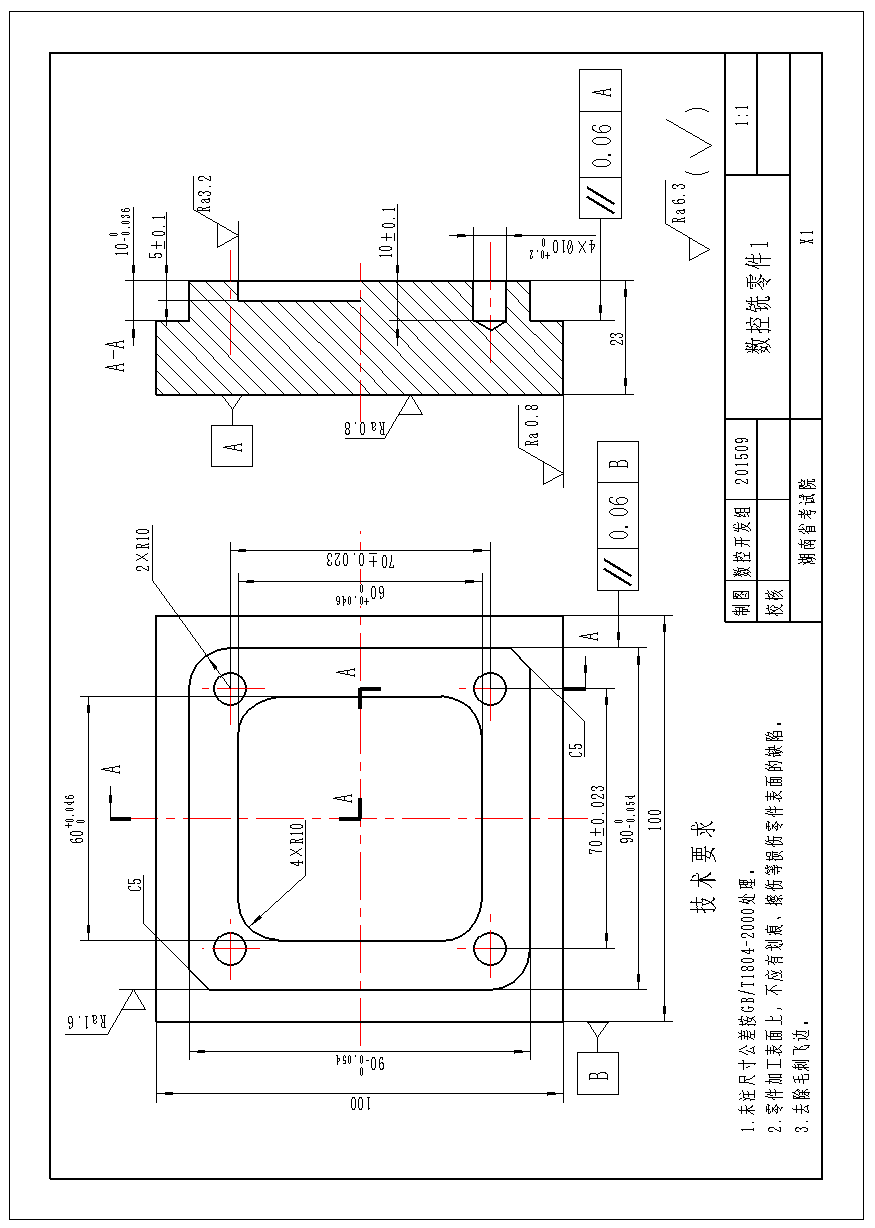
\includegraphics[width=0.9\linewidth]{images/1-1}
	\caption{}
	\label{fig:1-1}
\end{figure}
\begin{figure}
	\centering
	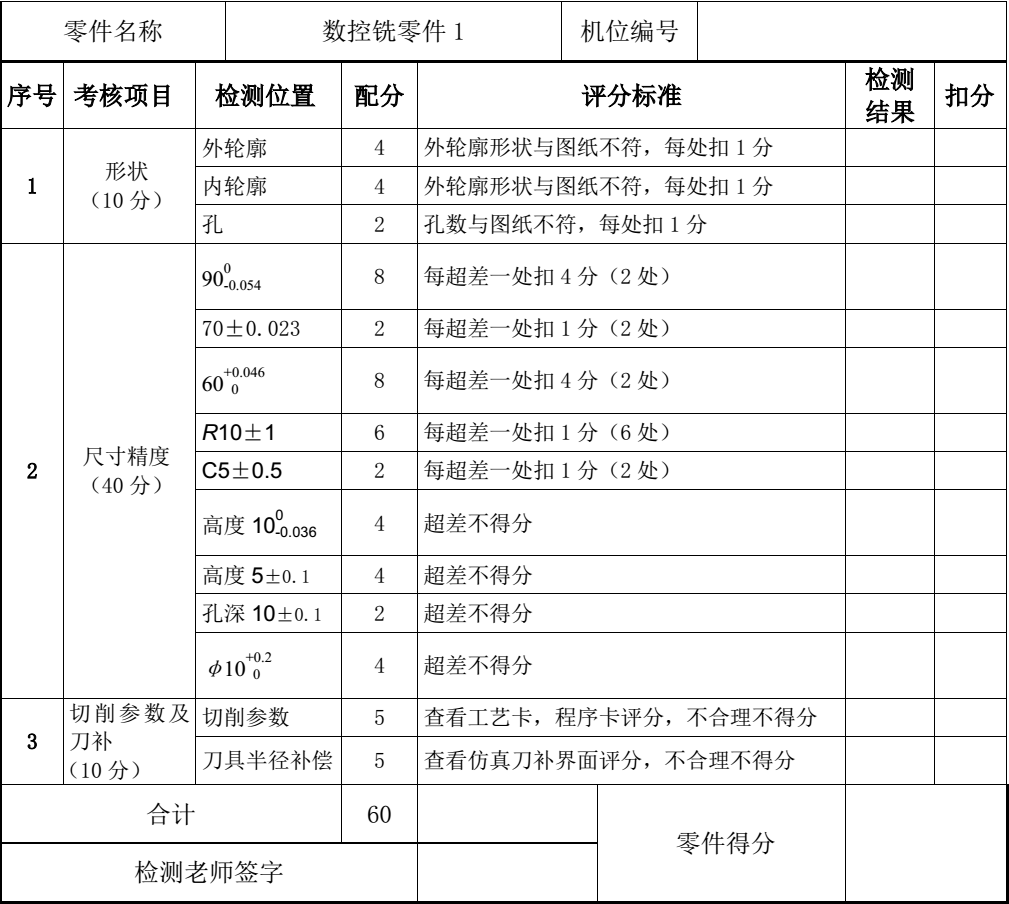
\includegraphics[width=0.9\linewidth]{images/1-2}
	\caption{}
	\label{fig:1-1}
\end{figure}
\begin{figure}
	\centering
	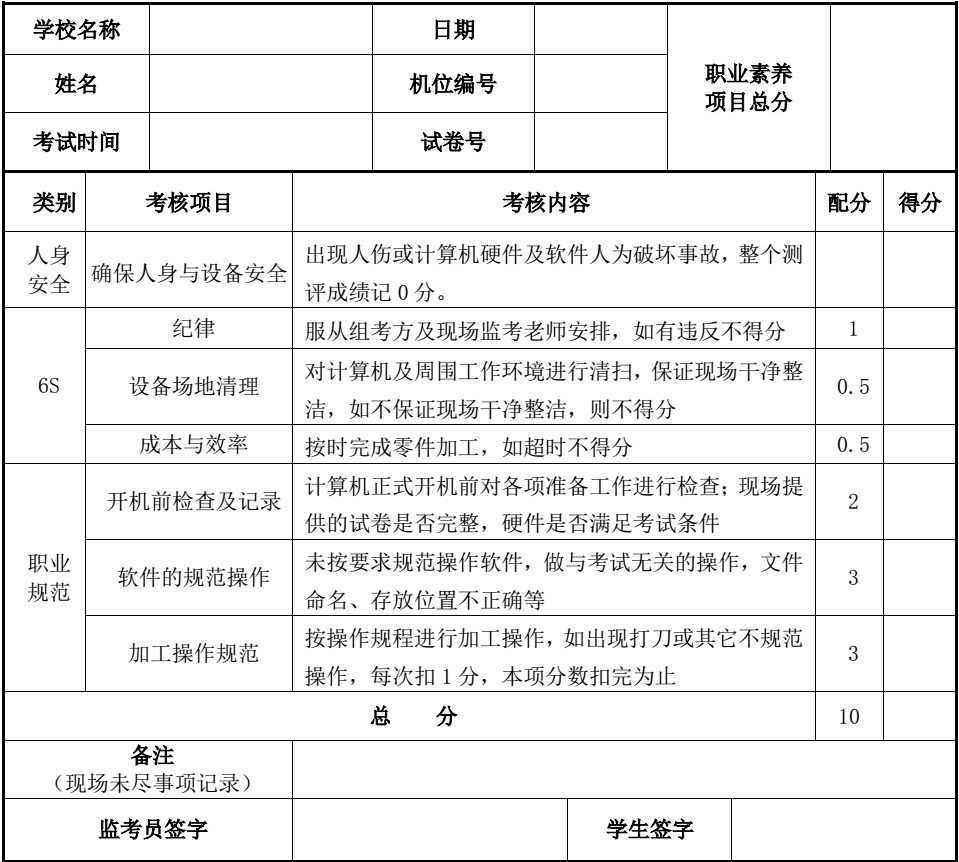
\includegraphics[width=0.9\linewidth]{images/1-3}
	\caption{}
	\label{fig:1-1}
\end{figure}
\begin{figure}
	\centering
	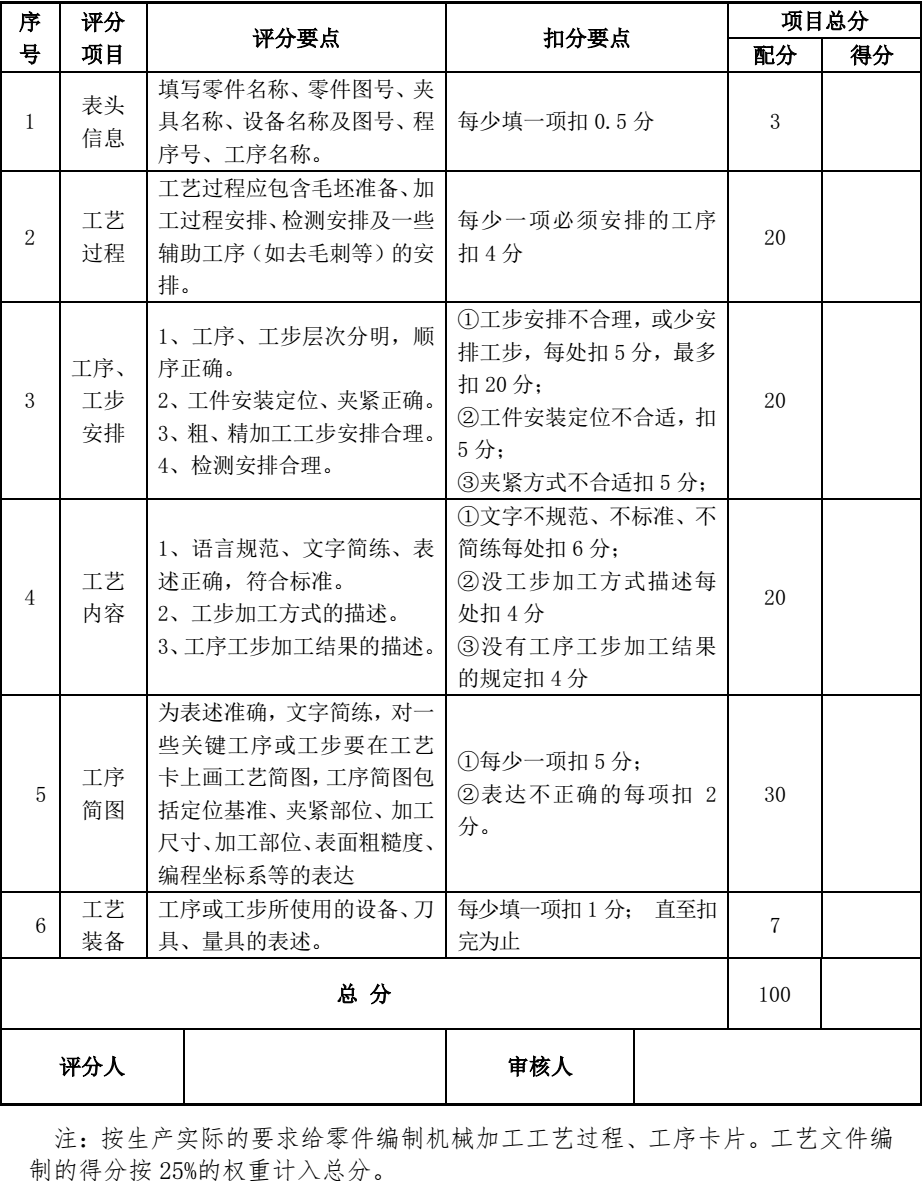
\includegraphics[width=0.9\linewidth]{images/1-4}
	\caption{}
	\label{fig:1-1}
\end{figure}
\begin{figure}
	\centering
	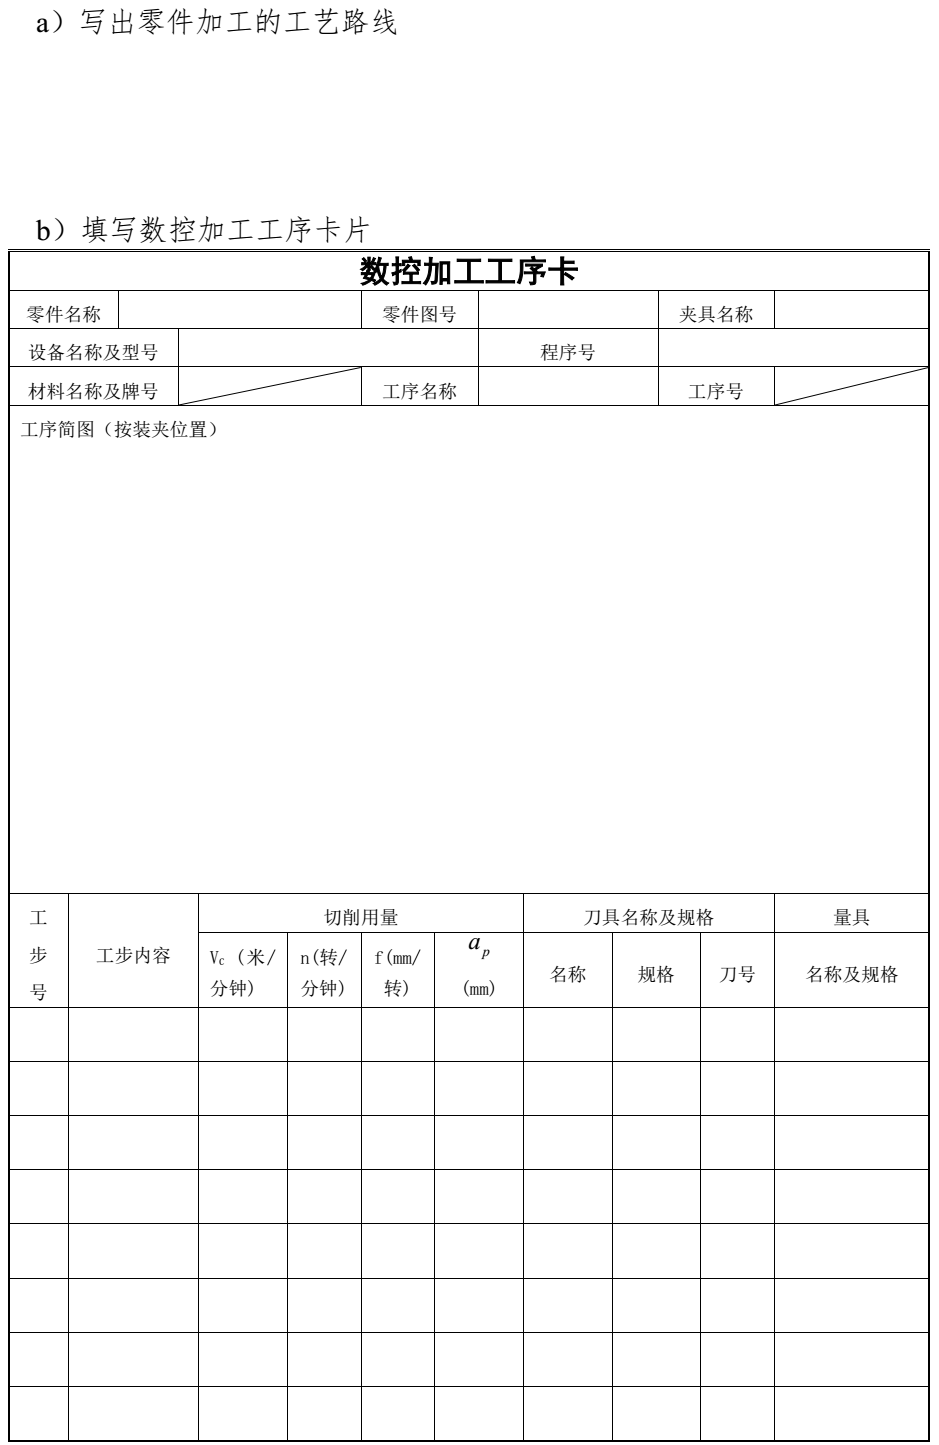
\includegraphics[width=0.9\linewidth]{images/1-5}
	\caption{}
	\label{fig:1-1}
\end{figure}
\begin{figure}
	\centering
	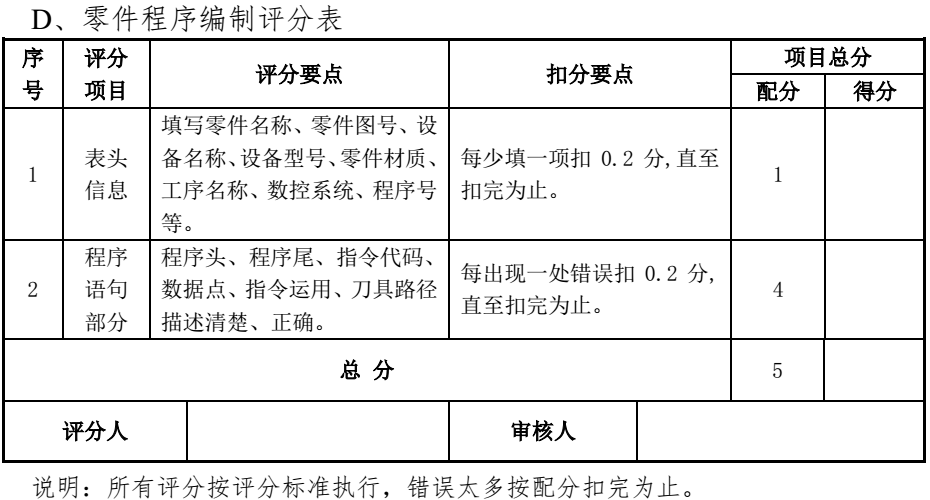
\includegraphics[width=0.9\linewidth]{images/1-6}
	\caption{}
	\label{fig:1-1}
\end{figure}
\begin{figure}
	\centering
	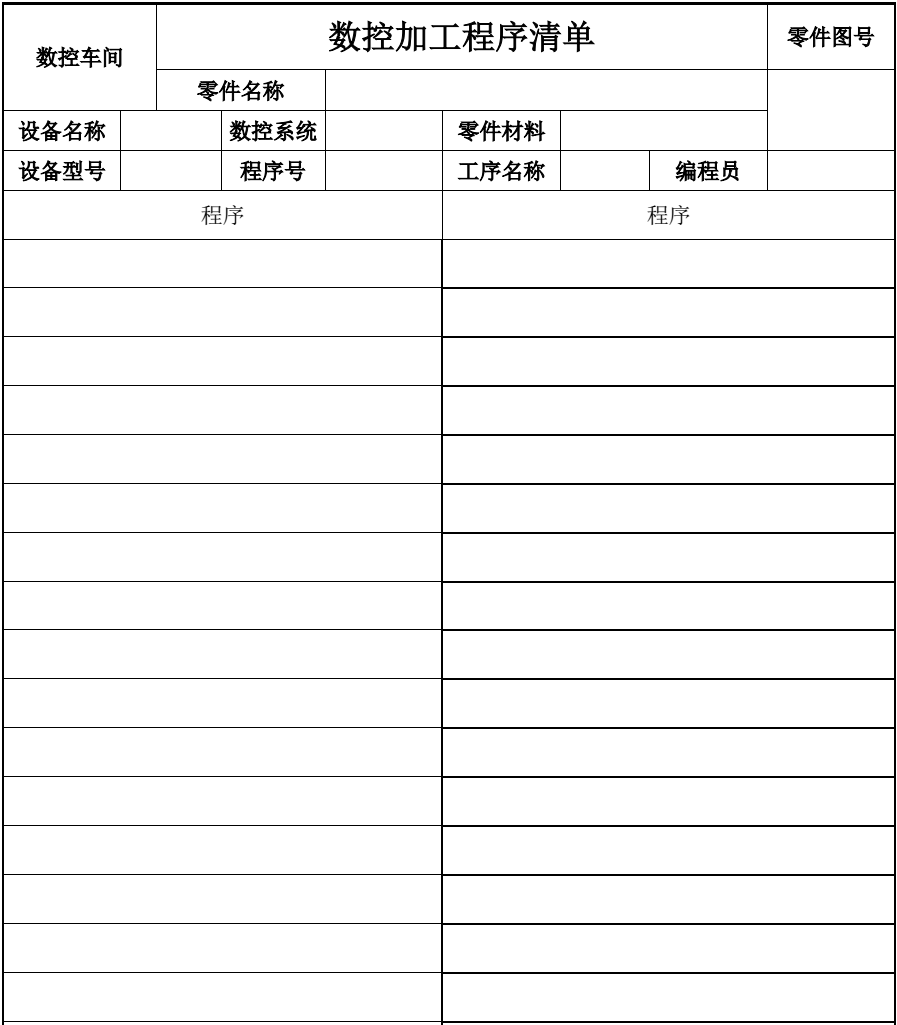
\includegraphics[width=0.9\linewidth]{images/1-7}
	\caption{}
	\label{fig:1-1}
\end{figure}
\begin{figure}
	\centering
	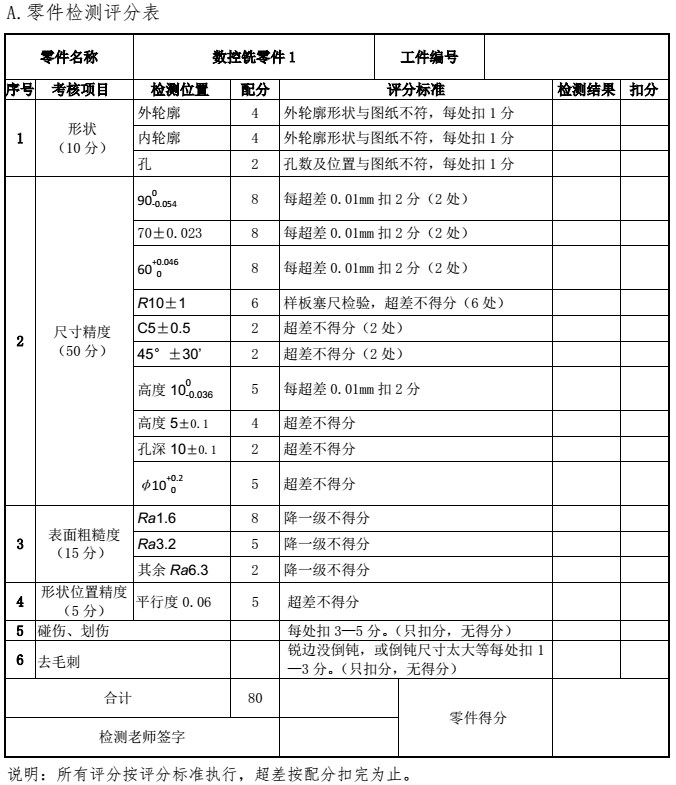
\includegraphics[width=0.9\linewidth]{images/1-8}
	\caption{}
	\label{fig:1-1}
\end{figure}
\begin{figure}
	\centering
	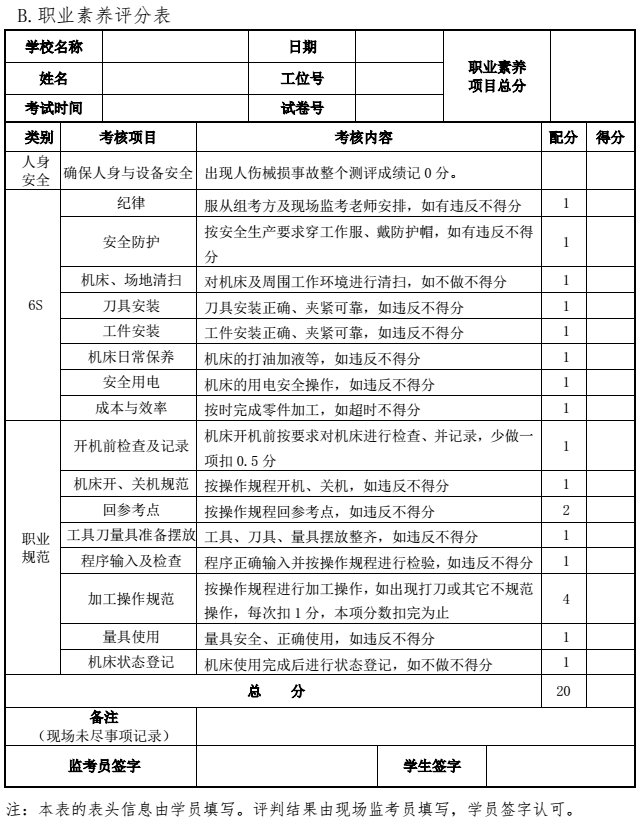
\includegraphics[width=0.9\linewidth]{images/1-9}
	\caption{}
	\label{fig:1-1}
\end{figure}